\documentclass{article}

\usepackage{graphicx}
\usepackage{tikz}
\usepackage{tikzsymbols}
\usetikzlibrary{calc,patterns,shapes.geometric}
\pagestyle{empty}
\usepackage[margin=0pt]{geometry}
\geometry{papersize={14in,12in}}

\def\centerarc[#1](#2)(#3:#4:#5){\draw[#1] ($(#2)+({#5*cos(#3)},{#5*sin(#3)})$) arc (#3:#4:#5);}

\begin{document}
	\begin{figure}
		\centering
		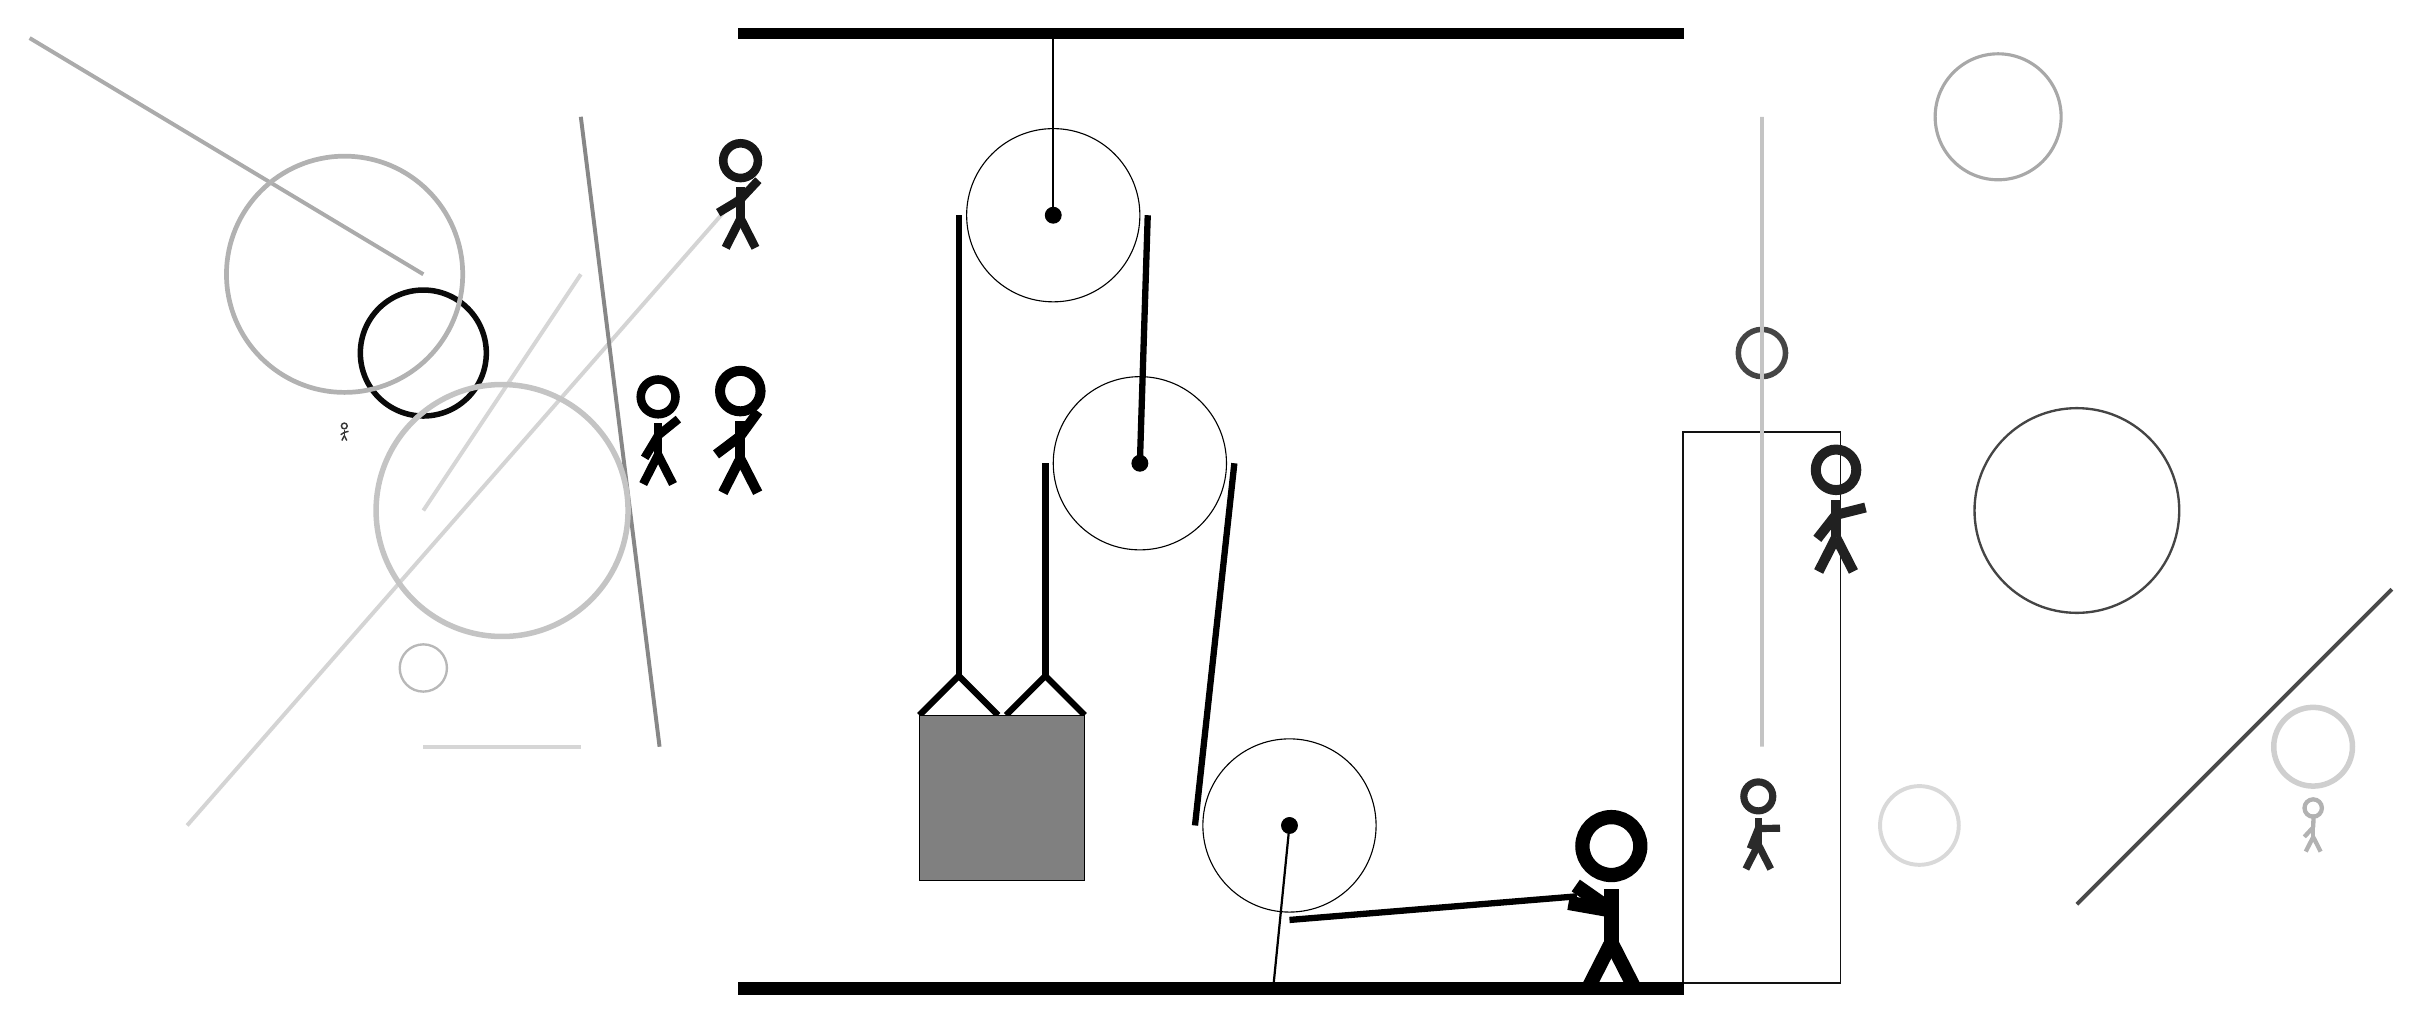
\begin{tikzpicture}
			%%%%% START %%%%%
			
			\draw[fill=black] (-2, 9) rectangle (10, 9.125);
			
			\draw (2, 6.75) circle (1.1);
			\draw[fill=black] (2, 6.75) circle (0.1);
			\draw[thick] (2, 6.75) -- (2, 9);
			
			\draw (3.1, 3.6) circle (1.1);
			\draw[fill=black] (3.1, 3.6) circle (0.1);
			
			\draw (5, -1) circle (1.1);
			\draw[fill=black] (5, -1) circle (0.1);
			\draw[thick] (5, -1) -- (4.8, -3);
			
			\node[line width=0.7mm, color=black!83] at (11, -1) {\Strichmaxerl[5][68][1]};
			
			\draw[line width=0.5mm, color=black!17](-2, 7) -- (-9, -1);
			\node[line width=0.3mm, color=black!91] at (-2, 7) {\Strichmaxerl[6][31][47]};
			\node[line width=0.6mm, color=black!79] at (-7, 4) {\Strichmaxerl[1][33][14]};
			\draw [line width=0.7mm, color=black!19](18, 0) circle (0.5);
			\draw[line width=0.2mm, color=black!93] (10, -3) rectangle (12, 4);
			\draw [line width=0.7mm, color=black!73](11, 5) circle (0.3);
			
			\draw [line width=0.3mm, color=black!28](-6, 1) circle (0.3);
			\node[line width=0.3mm, color=black!100] at (-3, 4) {\Strichmaxerl[6][59][39]};
			\draw [line width=0.7mm, color=black!96](-6, 5) circle (0.8);
			
			\draw[line width=0.5mm, color=black!33](-6, 6) -- (-11, 9);
			\draw[line width=0.5mm, color=black!47](-4, 8) -- (-3, 0);
			\draw[line width=0.5mm, color=black!16](-4, 6) -- (-6, 3);
			
			\node[line width=0.5mm, color=black!100] at (-2, 4) {\Strichmaxerl[7][37][54]};
			\node[line width=0.4mm, color=black!87] at (12, 3) {\Strichmaxerl[7][52][14]};
			\draw[line width=0.5mm, color=black!16](-4, 0) -- (-6, 0);
			\draw [line width=0.3mm, color=black!73](15, 3) circle (1.3);
			\draw [line width=0.7mm, color=black!23](-5, 3) circle (1.6);
			\draw[line width=0.5mm, color=black!23] (11, 0) rectangle (11, 8);
			\node[line width=0.4mm, color=black!30] at (18, -1) {\Strichmaxerl[3][47][88]};
			\draw [line width=0.6mm, color=black!30](-7, 6) circle (1.5);
			
			\draw [line width=0.4mm, color=black!34](14, 8) circle (0.8);
			
			\draw[line width=0.5mm, color=black!71](15, -2) -- (19, 2);
			\draw [line width=0.5mm, color=black!15](13, -1) circle (0.5);
			
			\draw[line width = 0.8mm]  (0.3, 0.4) -- (0.8, 0.9) -- (1.3, 0.4);
			\draw[line width = 0.8mm]  (1.4, 0.4) -- (1.9, 0.9) -- (2.4, 0.4);
			\draw[fill=black!50] (0.3, 0.4) rectangle (2.4, -1.7);
			
			\draw[line width = 0.8mm] (0.8, 6.75) -- (0.8, 0.9);
			\centerarc[line width = 0.8mm](2, 6.75)(0:180:1.2000000000000002);
			\draw[line width = 0.8mm] (3.2, 6.75) -- (3.1, 3.6);
			\draw[line width = 0.8mm] (1.9, 3.6) -- (1.9, 0.9);
			\centerarc[line width = 0.8mm](3.1, 3.6)(0:180:1.2000000000000002);
			\draw[line width = 0.8mm] (4.3, 3.6) -- (3.8, -1);
			\centerarc[line width = 0.8mm](5, -1)(180:270:1.2000000000000002);
			\draw[line width = 0.8mm] (5, -2.2) -- (8.65, -1.9);
			
			\node at (9, -2) {\Strichmaxerl[10][-35][170]};
			
			\draw[fill=black] (-2, -3) rectangle (10, -3.15);
			
			%%%%% END %%%%%
		\end{tikzpicture}
	\end{figure}	
\end{document}